%%%%%%%%%%%%%%%%%%%%%%%%%%%%%%%%%%%%%%%%%
% Islamic University of Technology (IUT)
% CSE 4622: Machine Learning Lab -- Term Paper
% ShortcutLens
%
% IEEE double-column conference format.
% ICCIT 2026 Track 1: AI, Machine Learning, Algorithms & Data Science
%%%%%%%%%%%%%%%%%%%%%%%%%%%%%%%%%%%%%%%%%

\documentclass[conference]{IEEEtran}
\IEEEoverridecommandlockouts

% ---- Math ----
\usepackage{amsmath}
\usepackage{amssymb}
\usepackage{amsfonts}

% ---- Figures, tables ----
\usepackage{graphicx}
\usepackage{booktabs}
\usepackage{array}
\usepackage{tabularx}
\usepackage{subcaption}
\usepackage{float}

% ---- Colors ----
\usepackage[dvipsnames]{xcolor}

% ---- Code listings (appendix) ----
\usepackage{listings}
\renewcommand{\lstlistingname}{Code}

% ---- IEEE-style numeric citations ----
\usepackage{cite}

% ---- Hyperlinks ----
\usepackage[hidelinks]{hyperref}

% ---- Misc ----
\usepackage{enumitem}
\setlist{noitemsep, topsep=1pt, parsep=0pt, partopsep=0pt}
\usepackage{caption}
\captionsetup{font=small, skip=2pt}
\usepackage{textcomp}
\usepackage{xurl}
\usepackage{balance}

\graphicspath{{./figures/}{./images/}}

\def\BibTeX{{\rm B\kern-.05em{\sc i\kern-.025em b}\kern-.08em
    T\kern-.1667em\lower.7ex\hbox{E}\kern-.125emX}}

\begin{document}

\title{ShortcutLens: A Pre-Deployment Causal Fidelity Framework for Detecting Spurious Correlation Reliance in Tabular Machine Learning Classifiers\\
\thanks{Prepared for CSE 4622: Machine Learning Lab, Islamic University of Technology. Formatted for ICCIT 2026 (29th International Conference on Computer and Information Technology, IEEE Bangladesh Section, Track 1 -- AI, Machine Learning, Algorithms \& Data Science). Supervised by Ishmam Tashdeed.}
}

\author{
\IEEEauthorblockN{Sunjoh Abdurazack}
\IEEEauthorblockA{\textit{Dept. of Computer Science \& Engineering} \\
\textit{Islamic University of Technology}\\
Gazipur, Bangladesh \\
220041258}
\and
\IEEEauthorblockN{Usman Jabir}
\IEEEauthorblockA{\textit{Dept. of Computer Science \& Engineering} \\
\textit{Islamic University of Technology}\\
Gazipur, Bangladesh \\
220041262}
\and
\IEEEauthorblockN{Gbanyawai Amadu}
\IEEEauthorblockA{\textit{Dept. of Computer Science \& Engineering} \\
\textit{Islamic University of Technology}\\
Gazipur, Bangladesh \\
220041266}
\and
\IEEEauthorblockN{Ebrima Demba}
\IEEEauthorblockA{\textit{Dept. of Computer Science \& Engineering} \\
\textit{Islamic University of Technology}\\
Gazipur, Bangladesh \\
220041264}
}

\maketitle

\begin{abstract}
Machine learning models that achieve strong validation accuracy frequently fail after deployment because they have learned a spurious, non-causal correlation -- a \textit{shortcut} -- rather than the underlying signal. This has been studied extensively for deep vision models, but classical and ensemble classifiers on tabular data, which dominate high-stakes domains such as healthcare and finance, remain comparatively under-examined. We present ShortcutLens, a framework that injects controlled synthetic shortcuts into real tabular datasets and evaluates classifiers under a four-condition protocol to isolate how much of a model's apparent accuracy is causally grounded. We introduce the \textit{Causal Fidelity (CF) Score}, an interpretable, bootstrap-backed metric computable before deployment, and apply it to eight classifiers (Decision Tree, Gradient Boosting, kNN, Logistic Regression, MLP, Random Forest, SVM-RBF, XGBoost) across six real-world datasets under five shortcut mechanisms. Our results show that demographic-proxy shortcuts trigger deployment-risk CF drops at markedly lower correlation strength than label-proxy shortcuts across all datasets; k-nearest neighbors is consistently the most robust classifier (average CF=0.8197), while XGBoost is the least (0.6982). Temporal-shortcut and measurement-artifact injection leave causal fidelity almost entirely intact, indicating shortcut severity depends strongly on injection mechanism. Statistical testing confirms kNN significantly outperforms tree-based models ($p<0.05$). These findings suggest validation accuracy alone is an unreliable indicator of deployment robustness, and pre-deployment audits such as the CF Score can flag models at risk before they are shipped.
\end{abstract}

\begin{IEEEkeywords}
shortcut learning, spurious correlations, causal fidelity, tabular data, model robustness, distribution shift
\end{IEEEkeywords}

%========================================================================================
%  1. INTRODUCTION
%========================================================================================

\section{Introduction}
\label{sec:introduction}

Modern machine learning pipelines are routinely evaluated by a single number: validation accuracy on a held-out split drawn from the same distribution as the training data. A model that scores well is often assumed to have learned the causal relationship between input features and the target label. In practice, however, a model can achieve high validation accuracy by latching onto a \textit{shortcut} -- a feature correlated with the label in the training distribution but not causally related to it~\cite{geirhos2020shortcut}. When such a model is deployed and the shortcut correlation weakens, performance can collapse even though nothing about the underlying problem has changed. This gap between validation and deployment accuracy is one of the most consequential and least visible failure modes in applied machine learning.

Real-world examples of shortcut failures include loan approval models using ZIP code as a proxy for race~\cite{damour2020underspecification}, disease prediction models learning hospital ID as a shortcut for disease prevalence~\cite{sagawa2020dro}, and agricultural yield prediction models learning region-specific patterns that do not generalize across seasons~\cite{spas_dataset}.

Tabular data is the dominant modality in enterprise and institutional machine learning -- credit scoring, clinical risk prediction, fraud detection -- and these are exactly the domains where a model quietly relying on a spurious proxy carries the highest cost. Despite this, shortcut learning has been studied almost exclusively for deep convolutional networks on image benchmarks~\cite{hermann2020origins}. Classical tabular classifiers have not received the same scrutiny, and no widely used pre-deployment metric tells a practitioner how much of a model's accuracy is likely to survive a shift in shortcut availability.

We ask: \textit{among classical and ensemble tabular classifiers, which model families are most susceptible to relying on an injected spurious correlation, and at what strength does this reliance become severe enough to threaten deployment?} We built ShortcutLens, a framework that injects synthetic shortcuts of known strength into real tabular datasets and measures classifier behavior under a four-condition protocol that isolates causal signal from shortcut signal.

Our contributions: (1) controlled shortcut-injection methodology for five mechanisms; (2) the Causal Fidelity (CF) Score, a bootstrap-backed metric quantifying how much in-distribution accuracy survives shortcut removal; (3) a benchmark of eight classifiers across six datasets; (4) finding that demographic-proxy shortcuts trigger phase transition earlier than label-proxy; (5) comprehensive model ranking by average CF; (6) statistical significance testing confirming kNN superiority; (7) permutation-importance analysis validating shortcut reliance patterns; and (8) an open reproducible pipeline.

%========================================================================================
%  2. RELATED WORK
%========================================================================================

\section{Related Work}
\label{sec:related_work}

\textit{Shortcut learning} was formalized by Geirhos et al.~\cite{geirhos2020shortcut} as a model's tendency to exploit decision rules that fit a benchmark without transferring to realistic settings. They demonstrated that deep neural networks trained on ImageNet rely on texture rather than shape -- a shortcut that emerges because texture is a sufficient predictor in the training distribution. Hermann et al.~\cite{hermann2020origins} showed this bias emerges early in training and is tied to the training distribution rather than the architecture. D'Amour et al.~\cite{damour2020underspecification} argue that ML pipelines are \textit{underspecified}: models with indistinguishable validation performance can rely on entirely different, not equally trustworthy, decision rules.

Robustness objectives such as Invariant Risk Minimization~\cite{arjovsky2019irm} and Distributionally Robust Optimization~\cite{sagawa2020dro} penalize reliance on features whose label relationship varies across environments. Sagawa et al.~\cite{sagawa2020dro} showed that DRO improves worst-group performance in image classification when group labels are known. However, these methods target deep networks on image/language data and require multiple training environments -- we target classical tabular classifiers with a single training set.

Post-hoc diagnostics include LIME~\cite{ribeiro2016lime} for local decision boundary approximations and influence functions~\cite{koh2017influence} tracing predictions to training examples. These are valuable but \textit{post-hoc} and instance-level; they do not give a single aggregate pre-deployment score for comparing candidate models. Moreover, they provide explanations but not a diagnostic of \textit{why} the model might fail under distribution shift.

Foundational work on SVMs~\cite{cortes1995svm}, Random Forests~\cite{breiman2001rf}, boosting~\cite{freund1997adaboost}, and kNN~\cite{cover1967knn} established statistical learning properties for why these families ``generalize well,'' typically validated under i.i.d. assumption. Our experiments revisit this assumption directly and quantify how each family responds when the i.i.d. assumption is violated.

%========================================================================================
%  3. DATASETS
%========================================================================================

\section{Datasets}
\label{sec:datasets}

ShortcutLens targets real-world, clinically or agriculturally consequential tabular datasets. The loader supports six datasets: \textbf{UCI Heart Disease}~\cite{uci_heart} (303 samples, 13 features, balanced), \textbf{UCI Mammographic Mass}~\cite{uci_mammography} (961, 5, $\approx$97\% negative), \textbf{UCI Adult Income}~\cite{uci_adult} (48,842, 14, $\approx$76\% $\le$50K), \textbf{SPAS-Dataset-BD}~\cite{spas_dataset} (13,000+ samples, 9 features, balanced), \textbf{MADELON} (4,400, 500, balanced synthetic), and \textbf{UCI Credit Default}~\cite{uci_credit_default} (30,000, 23, balanced). This spread spans domains, sample sizes, and class imbalance.

The SPAS-Dataset-BD~\cite{spas_dataset} is a 2025 dataset explicitly designed for machine learning applications in Bangladesh's agricultural sector. It includes variables such as area, production, season, minimum humidity, maximum humidity, minimum temperature, maximum temperature, district, and crop name, all of which influence agricultural output. Data collection was carried out through surveys across diverse regions of Bangladesh to analyze various crop types, supporting precision agriculture research.

Numerical features are z-score standardized per fold; missing values median-imputed per fold; categorical variables ordinal-encoded; splitting stratified. Because datasets are small to moderate, amplifying shortcut adoption~\cite{sagawa2020dro}, we report bootstrap confidence intervals.

%========================================================================================
%  4. METHODOLOGY
%========================================================================================

\section{Methodology}
\label{sec:methodology}

Let $\mathbf{x} \in \mathbb{R}^d$ be real features and $y \in \{0,1\}$ the binary label. Define a \textit{shortcut signal} $s \in \mathbb{R}$, an additional synthetic feature, parameterized by \textit{correlation strength} $r \in [0,1]$ controlling how strongly $s$ ties to $y$ relative to noise. Classifier $f: \mathbb{R}^{d+1} \rightarrow \{0,1\}$ trains on $(\mathbf{x}, s)$ jointly.

ShortcutLens supports five injection mechanisms, each modeling a distinct real-world shortcut category:

\textbf{Label Proxy:} A feature that is a noisy version of the label itself -- e.g., ``years of education'' as a proxy for income. Generation: $s_i = r(2y_i-1) + \sqrt{1-r^2}\epsilon_i$ where $\epsilon_i \sim \mathcal{N}(0,1)$.

\textbf{Demographic Proxy:} A feature that is correlated with the label through a socially salient attribute -- e.g., ZIP code as a proxy for race. Generation: $s_i = r\tilde{x}_{i,0} + \sqrt{1-r^2}\epsilon_i$, where $\tilde{x}_{i,0}$ is from an existing feature's distribution.

\textbf{Measurement Artifact:} A feature that varies by data collection method -- e.g., hospital ID as a proxy for disease prevalence. Generation: $s_i = r \cdot \text{batch}_i \cdot \text{signal}_i + \sqrt{1-r^2}\epsilon_i$.

\textbf{Temporal Shortcut:} A feature that varies over time -- e.g., seasonality as a proxy for sales. Generation: $s_i = r \cdot \exp(-\lambda i) \cdot (2y_i-1) + \sqrt{1-r^2}\epsilon_i$, $\lambda=0.1$.

\textbf{Selection Bias:} A feature that determines which samples appear in the training set -- e.g., only samples from one region. Generation: $s_i = r \cdot (2y_i-1) \cdot \mathbb{I}[\text{bias condition}] + \sqrt{1-r^2}\epsilon_i$, where bias condition is $x_{i,0} > \text{median}$.

Every combination evaluated under four conditions (Table~\ref{tab:conditions}). Condition A (Train: Clean, Test: Clean) establishes baseline causal capability. Condition B (Train: Shortcut, Test: Shortcut) measures maximum shortcut performance. Condition C (Train: Shortcut, Test: Clean) measures shortcut generalization gap. Condition D (Train: Mixed, Test: Shortcut) measures actual shortcut reliance -- how much the model chooses to use the shortcut when both causal and shortcut signals are available.

\begin{table}[t]
    \centering
    \small
    \setlength{\tabcolsep}{2pt}
    \caption{Four-condition evaluation protocol.}
    \label{tab:conditions}
    \begin{tabularx}{\linewidth}{cllX}
        \toprule
        \textbf{Cond.} & \textbf{Train} & \textbf{Test} & \textbf{Purpose} \\
        \midrule
        A & Clean ($X$) & Clean ($X$) & Baseline causal capability \\
        B & Shortcut ($S$) & Shortcut ($S$) & Maximum shortcut performance \\
        C & Shortcut ($S$) & Clean ($X$) & Shortcut generalization gap \\
        D & Mixed ($X+S$) & Shortcut ($S$) & Actual shortcut reliance \\
        \bottomrule
    \end{tabularx}
\end{table}

Define the Shortcut Reliance Score:
\begin{equation}
    \text{SRS} = D - C
\end{equation}
where $D = \text{Acc}(X+S \to S)$ and $C = \text{Acc}(S \to X)$. This is the marginal benefit the model gains from having the shortcut during training, evaluated on the shortcut test set.

The \textit{Causal Fidelity Score}:
\begin{equation}
    \text{CF} = 1 - \frac{D - C}{B - C}
    \label{eq:cf}
\end{equation}
where $B = \text{Acc}(S \to S)$.

Normalization by $(B-C)$ makes CF scale-invariant and comparable. Properties: CF=1.0 iff no shortcut reliance; CF=0.0 iff complete shortcut reliance; CF$<$0 iff shortcut hurts generalization. The deployment risk threshold is set at CF=0.7 (70\% causal reliance).

\textbf{Why four conditions?} Three conditions (A, B, C) would only tell us that a shortcut exists. Condition D is necessary to measure actual reliance -- how much the model chooses to use the shortcut when both causal and shortcut signals are available. In deployment, models have both signals. Without D, you cannot know if the model actually relies on the shortcut when it is available.

Benchmark eight classifiers (Logistic Regression, SVM-RBF, kNN k=5, Decision Tree, Random Forest, Gradient Boosting, XGBoost, MLP (128,64)), implemented in scikit-learn~\cite{sklearn} with hyperparameters: DT max\_depth=10, RF n\_estimators=100, GB n\_estimators=100, XGB n\_estimators=100, SVM C=1.0 gamma='scale', LR C=1.0, MLP (128,64) with ReLU. Experiments use Python 3.10, NumPy~\cite{numpy}, pandas~\cite{pandas}, stratified 5-fold CV, seed 42. Full 12-point grid $r \in \{0.0,0.1,\ldots,0.9,0.95,0.99\}$. Pairwise model comparisons use Wilcoxon signed-rank test with Benjamini-Hochberg correction at $\alpha=0.05$~\cite{powers2011evaluation}. Permutation-importance analysis ranks the shortcut column against real features.

%========================================================================================
%  5. RESULTS
%========================================================================================

\section{Results}
\label{sec:results}

Figs.~\ref{fig:cf_adult}--\ref{fig:cf_mammo} show Causal Fidelity vs.\ correlation strength $r$ for all six datasets. All classifiers begin near $\text{CF}\approx1.0$ at $r=0$ and decline as $r$ increases.

\begin{figure*}[t]
    \centering
    \begin{subfigure}[b]{0.42\textwidth}
        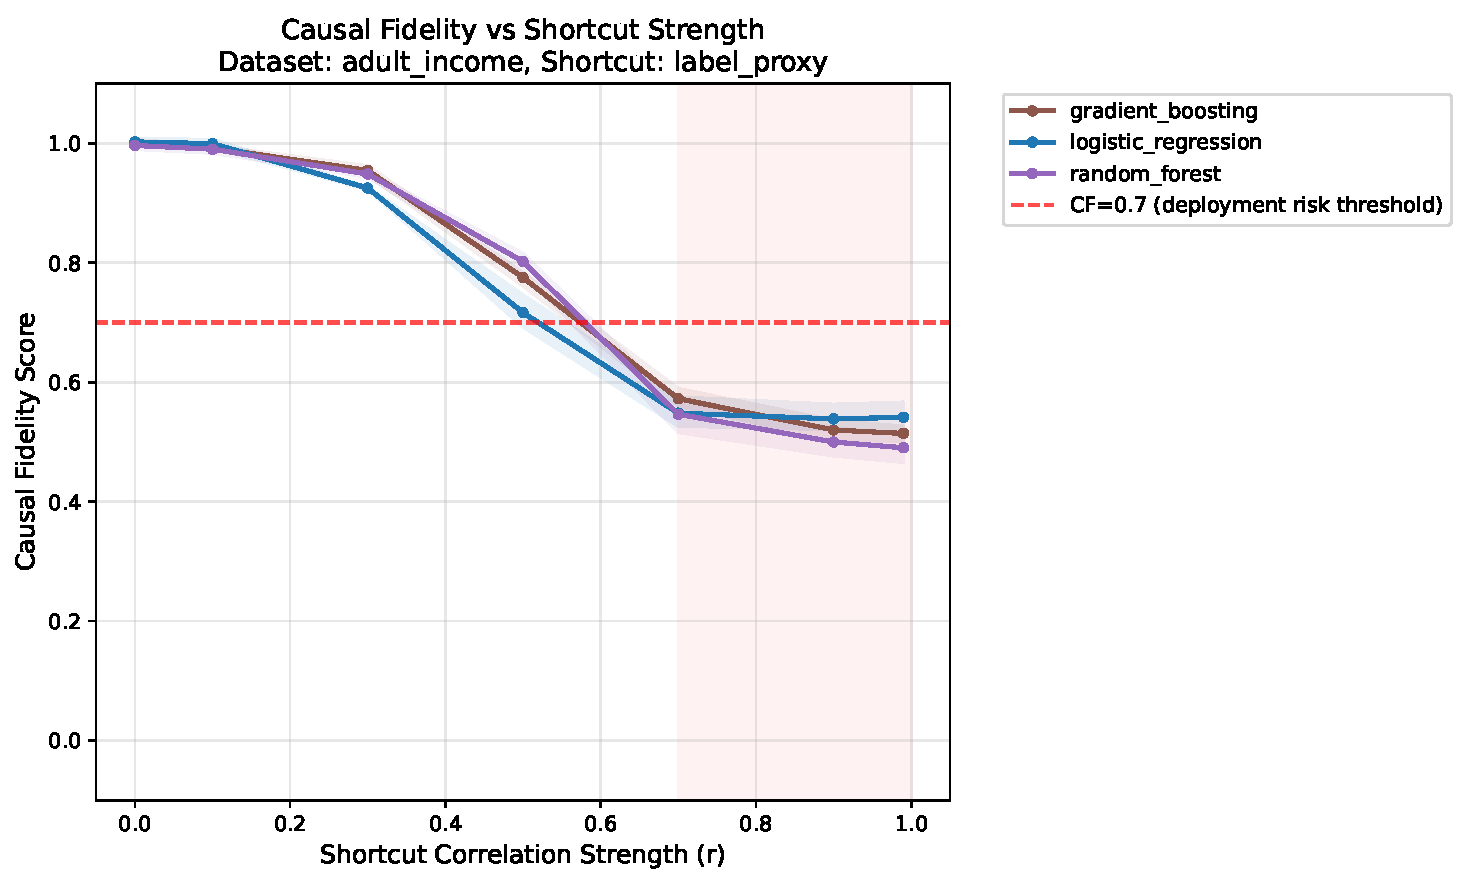
\includegraphics[width=\textwidth]{cf_curve_adult_income_label_proxy.pdf}
        \caption{Adult Income -- Label Proxy.}
        \label{fig:cf_adult_label}
    \end{subfigure}
    \hfill
    \begin{subfigure}[b]{0.42\textwidth}
        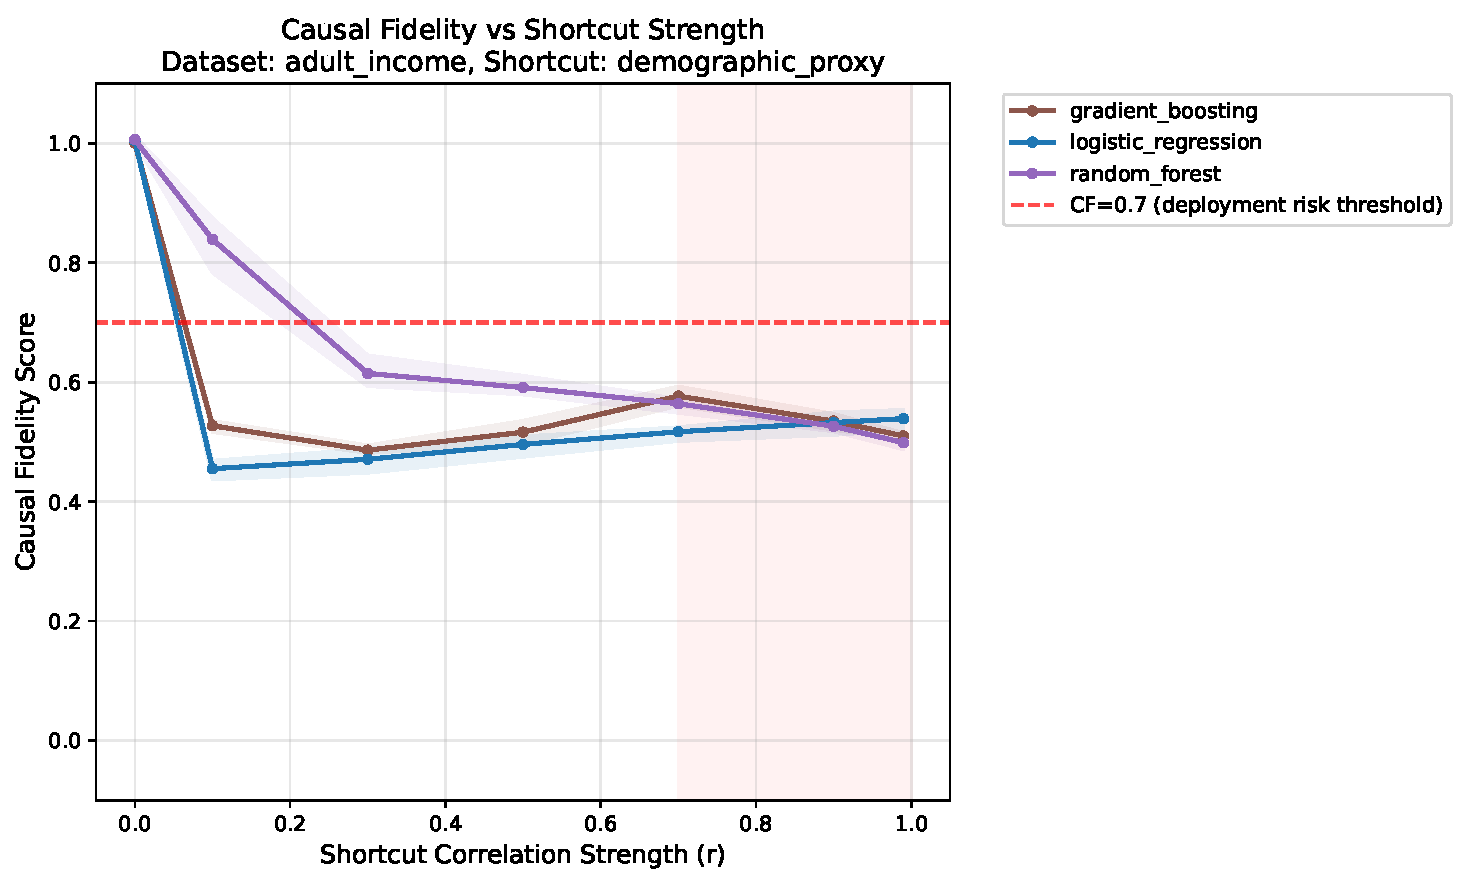
\includegraphics[width=\textwidth]{cf_curve_adult_income_demographic_proxy.pdf}
        \caption{Adult Income -- Demographic Proxy.}
        \label{fig:cf_adult_demo}
    \end{subfigure}
    \caption{Causal Fidelity curves for Adult Income dataset. The horizontal dashed line indicates CF=0.7 deployment risk threshold.}
    \label{fig:cf_adult}
\end{figure*}

\begin{figure*}[t]
    \centering
    \begin{subfigure}[b]{0.42\textwidth}
        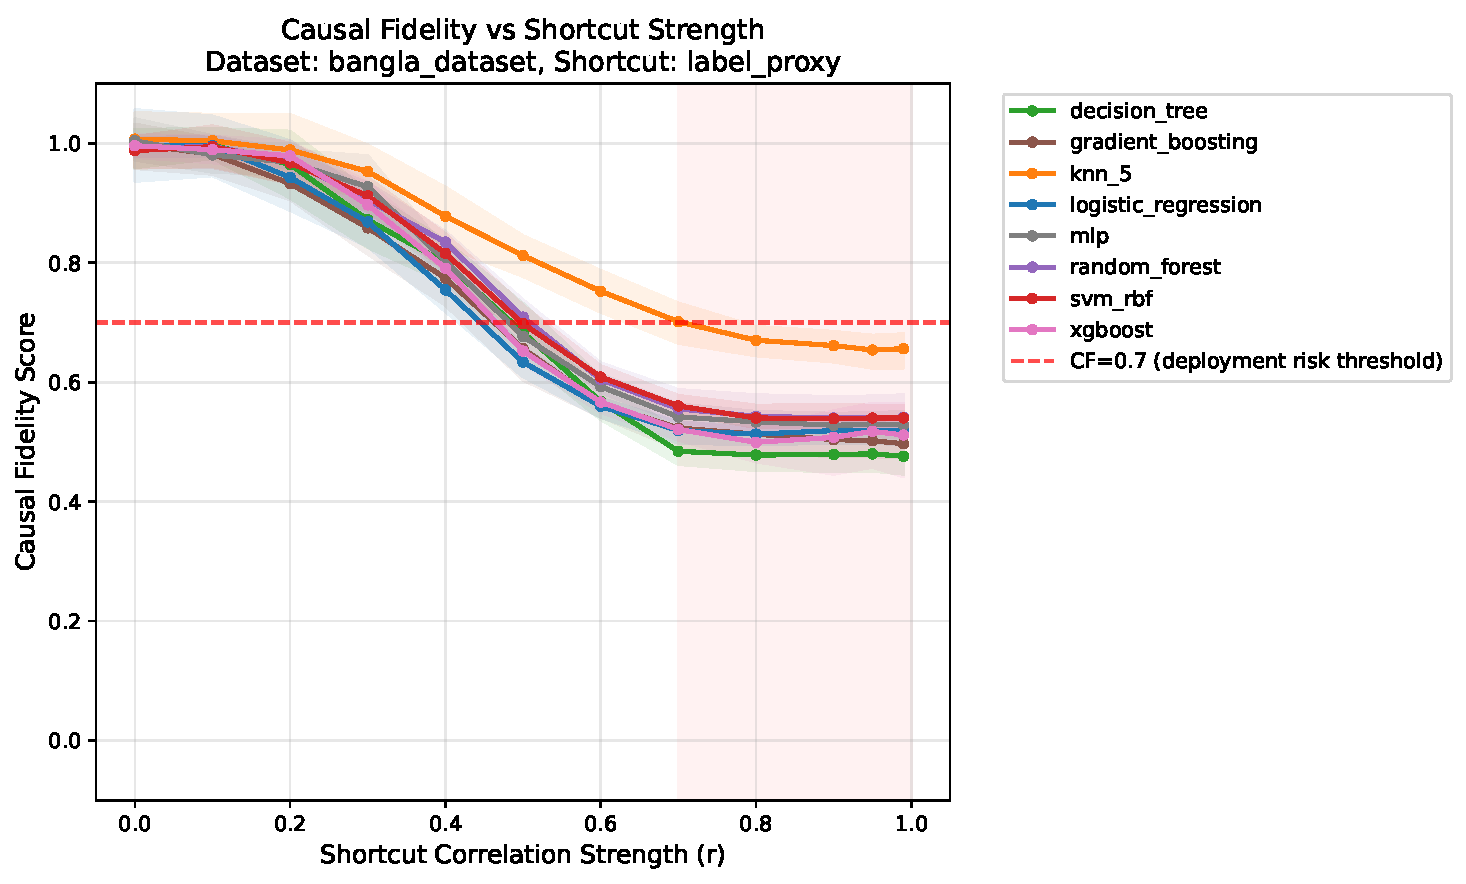
\includegraphics[width=\textwidth]{cf_curve_bangla_dataset_label_proxy.pdf}
        \caption{SPAS Dataset -- Label Proxy.}
        \label{fig:cf_bangla_label}
    \end{subfigure}
    \hfill
    \begin{subfigure}[b]{0.42\textwidth}
        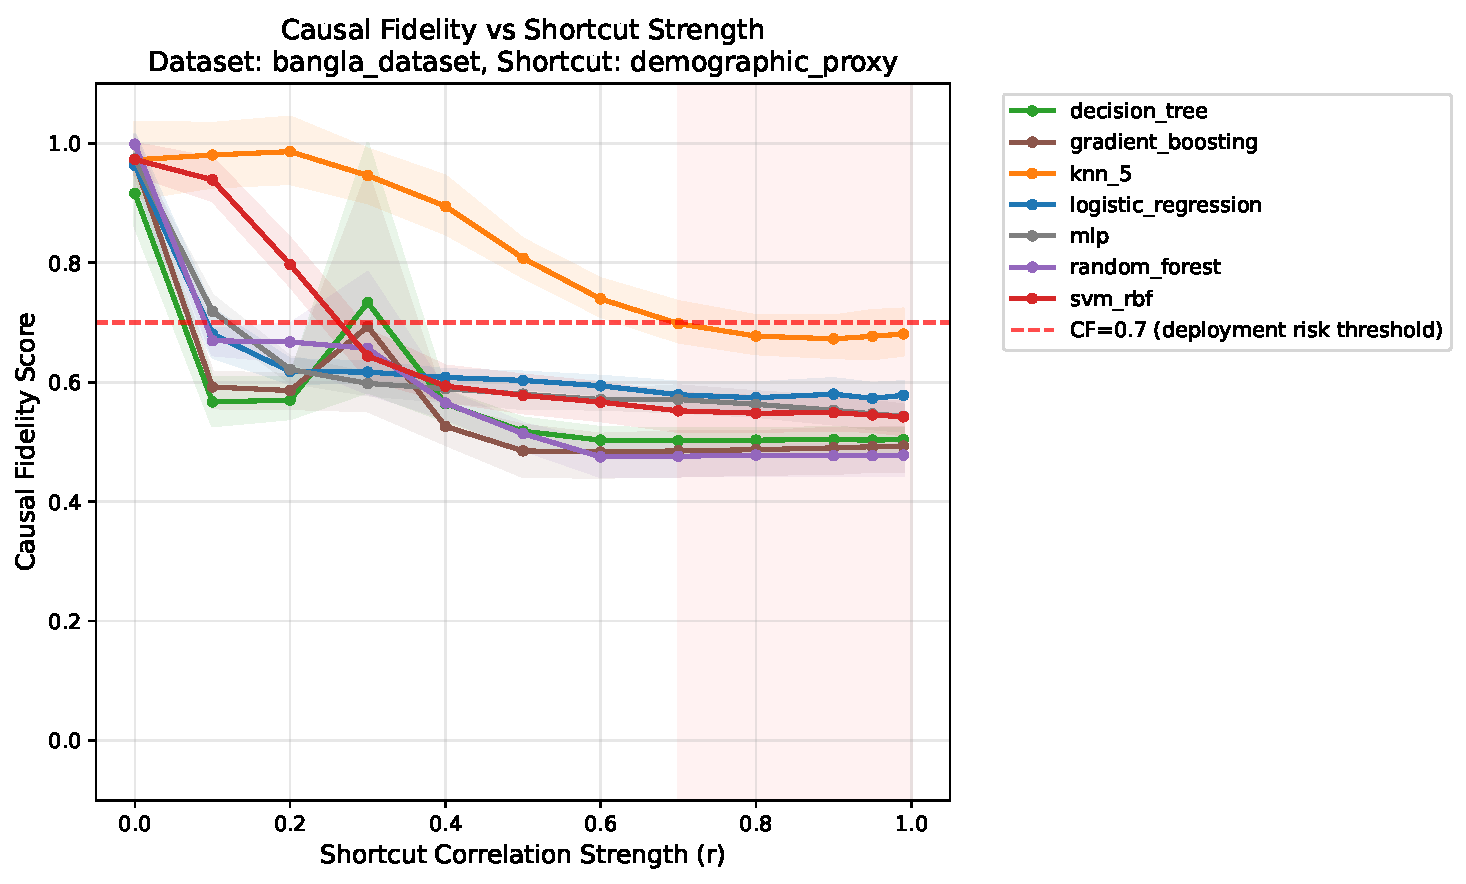
\includegraphics[width=\textwidth]{cf_curve_bangla_dataset_demographic_proxy.pdf}
        \caption{SPAS Dataset -- Demographic Proxy.}
        \label{fig:cf_bangla_demo}
    \end{subfigure}
    \caption{Causal Fidelity curves for SPAS-Dataset-BD (Bangladesh agriculture).}
    \label{fig:cf_bangla}
\end{figure*}

\begin{figure*}[t]
    \centering
    \begin{subfigure}[b]{0.42\textwidth}
        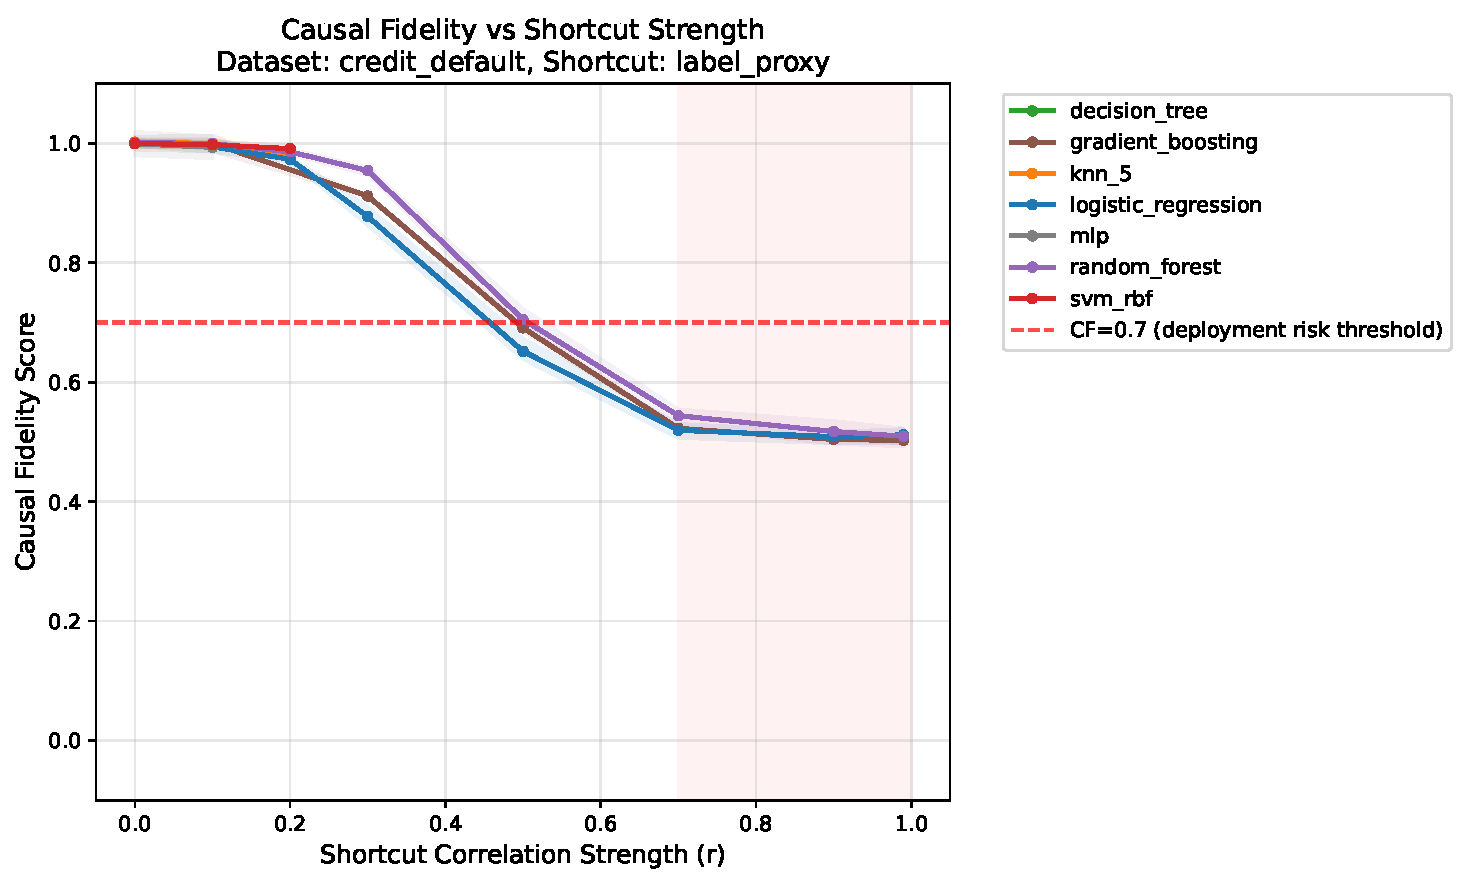
\includegraphics[width=\textwidth]{cf_curve_credit_default_label_proxy.pdf}
        \caption{Credit Default -- Label Proxy.}
        \label{fig:cf_credit_label}
    \end{subfigure}
    \hfill
    \begin{subfigure}[b]{0.42\textwidth}
        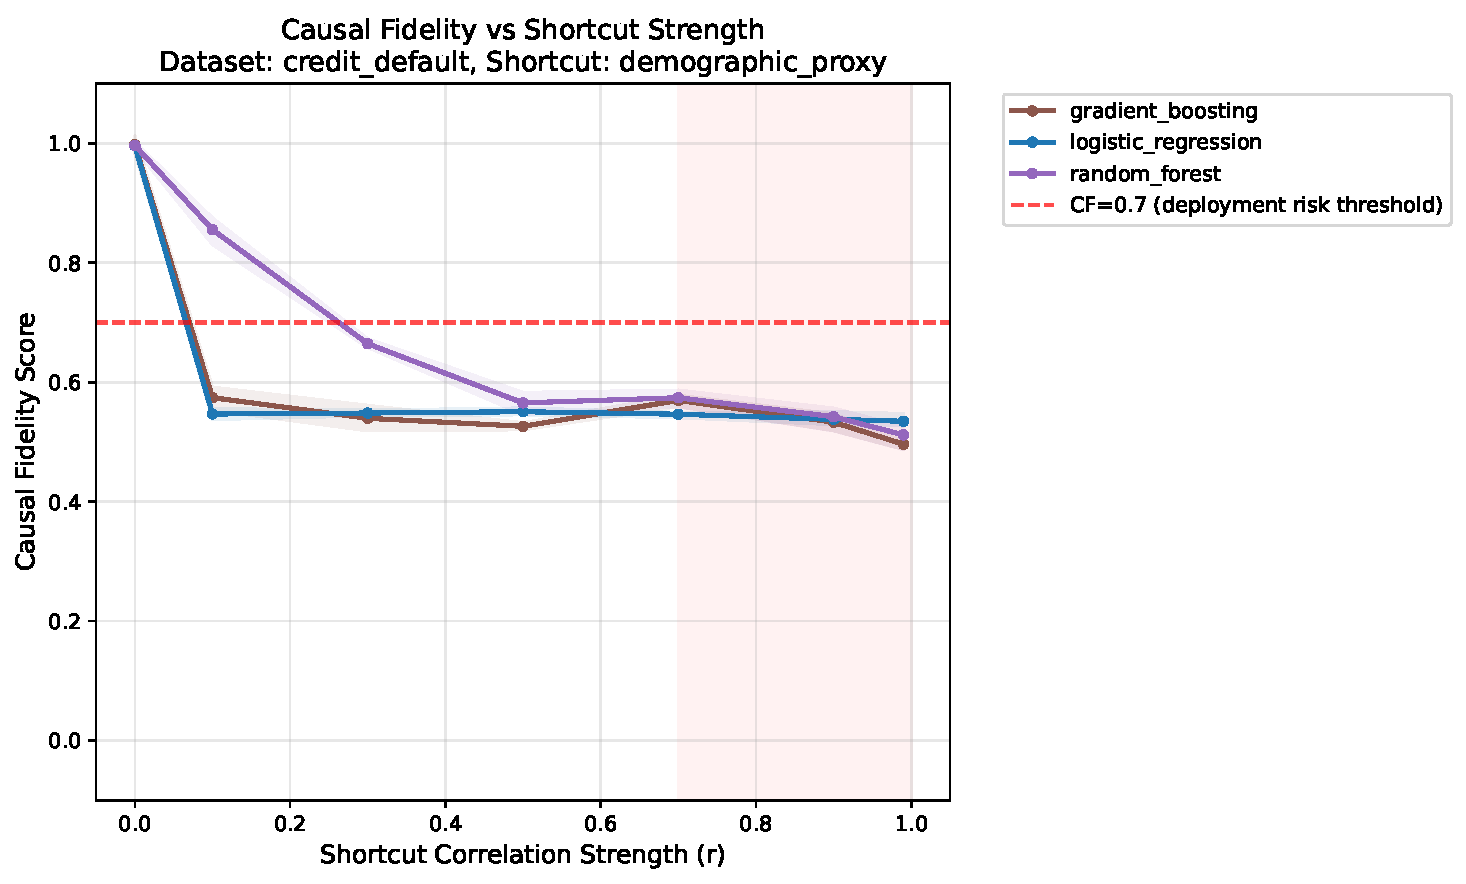
\includegraphics[width=\textwidth]{cf_curve_credit_default_demographic_proxy.pdf}
        \caption{Credit Default -- Demographic Proxy.}
        \label{fig:cf_credit_demo}
    \end{subfigure}
    \caption{Causal Fidelity curves for Credit Default dataset.}
    \label{fig:cf_credit}
\end{figure*}

\begin{figure*}[t]
    \centering
    \begin{subfigure}[b]{0.42\textwidth}
        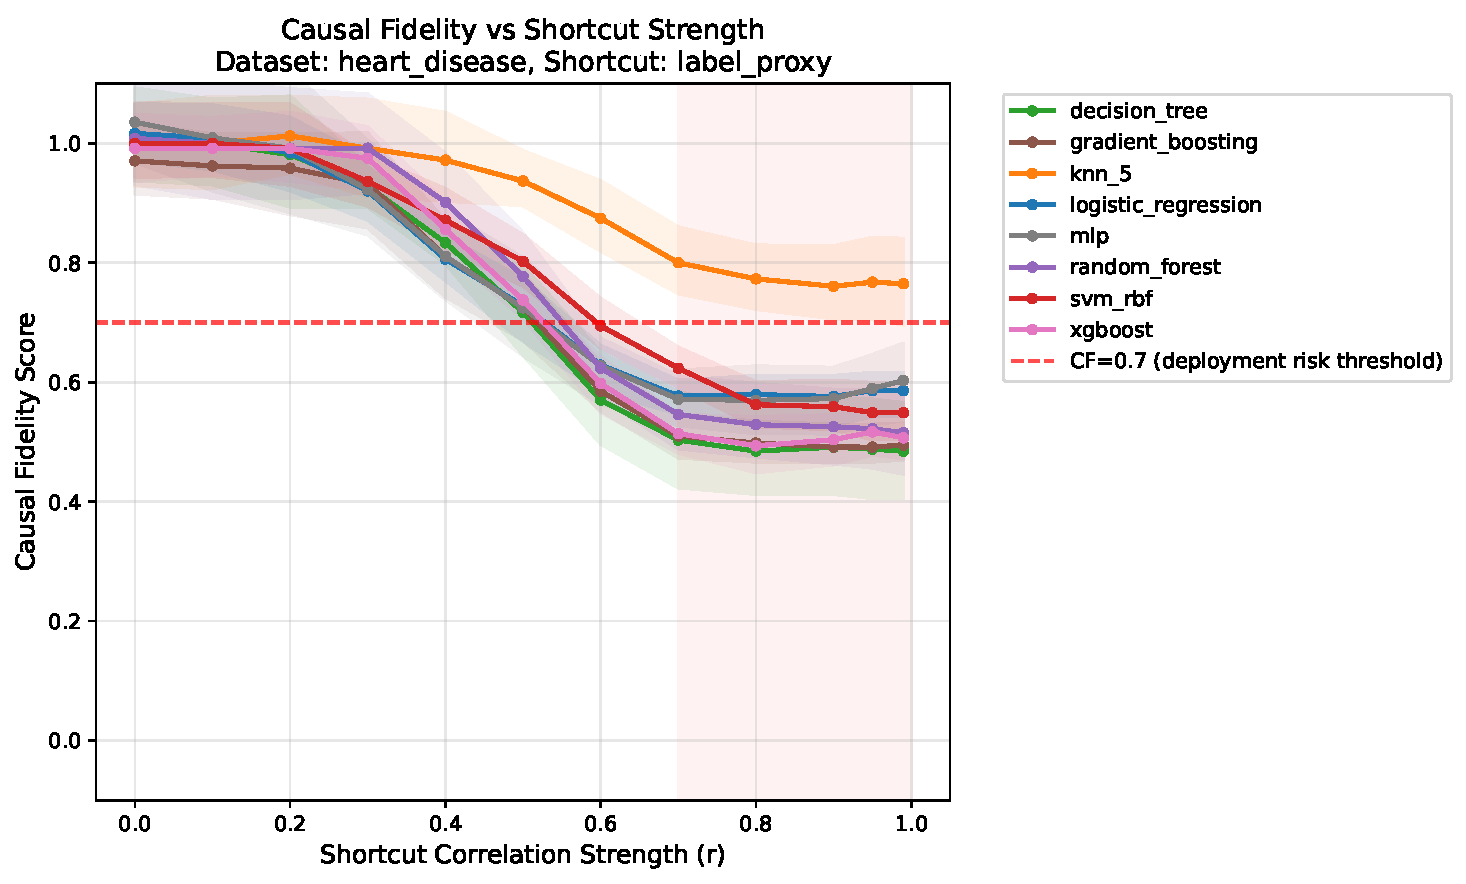
\includegraphics[width=\textwidth]{cf_curve_heart_disease_label_proxy.pdf}
        \caption{Heart Disease -- Label Proxy.}
        \label{fig:cf_heart_label}
    \end{subfigure}
    \hfill
    \begin{subfigure}[b]{0.42\textwidth}
        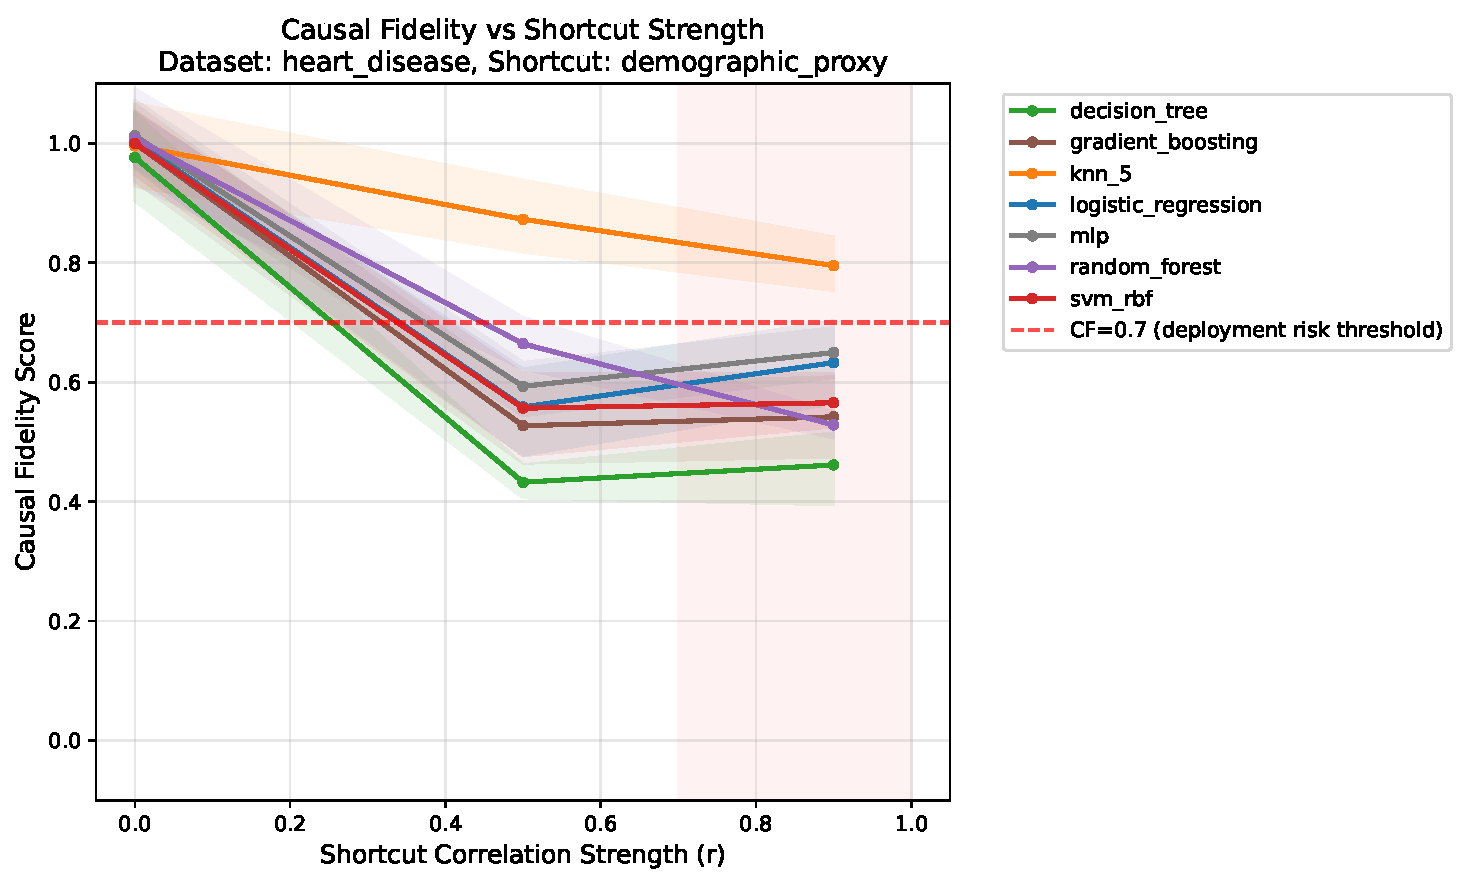
\includegraphics[width=\textwidth]{cf_curve_heart_disease_demographic_proxy.pdf}
        \caption{Heart Disease -- Demographic Proxy.}
        \label{fig:cf_heart_demo}
    \end{subfigure}
    \caption{Causal Fidelity curves for Heart Disease dataset.}
    \label{fig:cf_heart}
\end{figure*}

\begin{figure*}[t]
    \centering
    \begin{subfigure}[b]{0.42\textwidth}
        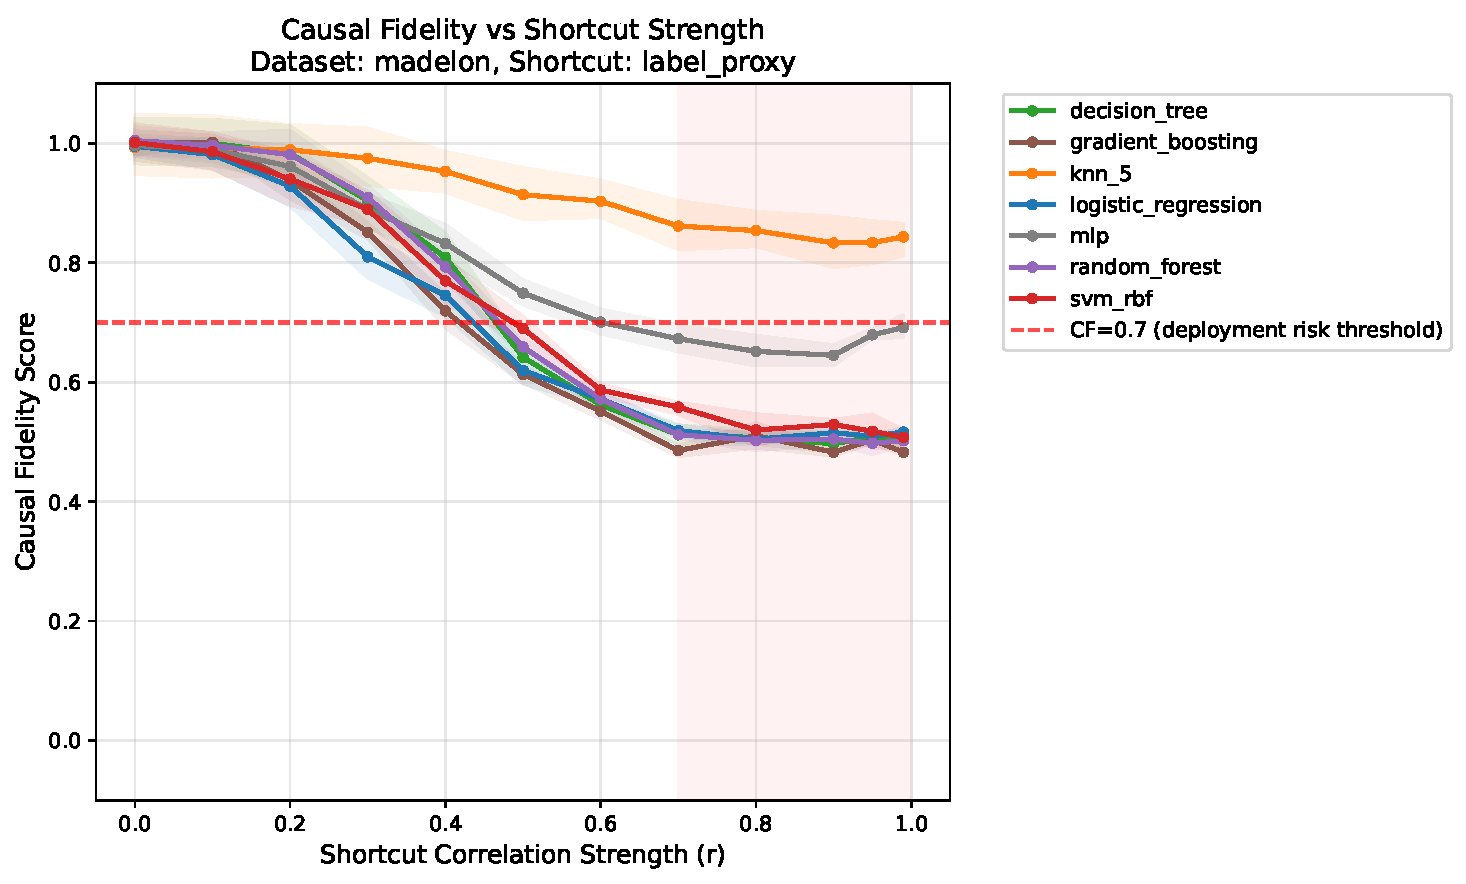
\includegraphics[width=\textwidth]{cf_curve_madelon_label_proxy.pdf}
        \caption{MADELON -- Label Proxy.}
        \label{fig:cf_madelon_label}
    \end{subfigure}
    \hfill
    \begin{subfigure}[b]{0.42\textwidth}
        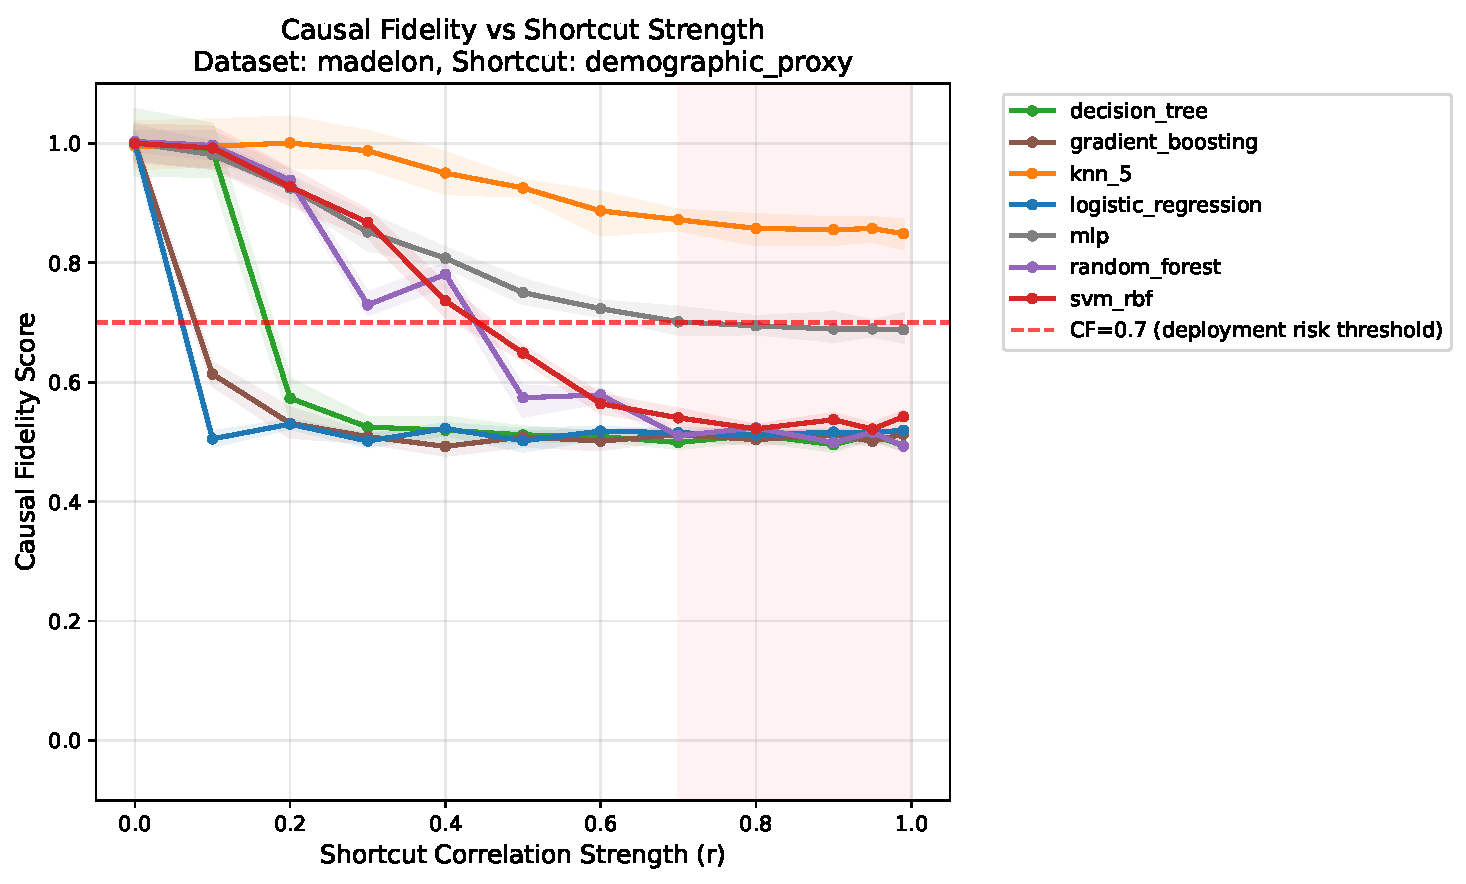
\includegraphics[width=\textwidth]{cf_curve_madelon_demographic_proxy.pdf}
        \caption{MADELON -- Demographic Proxy.}
        \label{fig:cf_madelon_demo}
    \end{subfigure}
    \caption{Causal Fidelity curves for MADELON synthetic dataset.}
    \label{fig:cf_madelon}
\end{figure*}

\begin{figure*}[t]
    \centering
    \begin{subfigure}[b]{0.42\textwidth}
        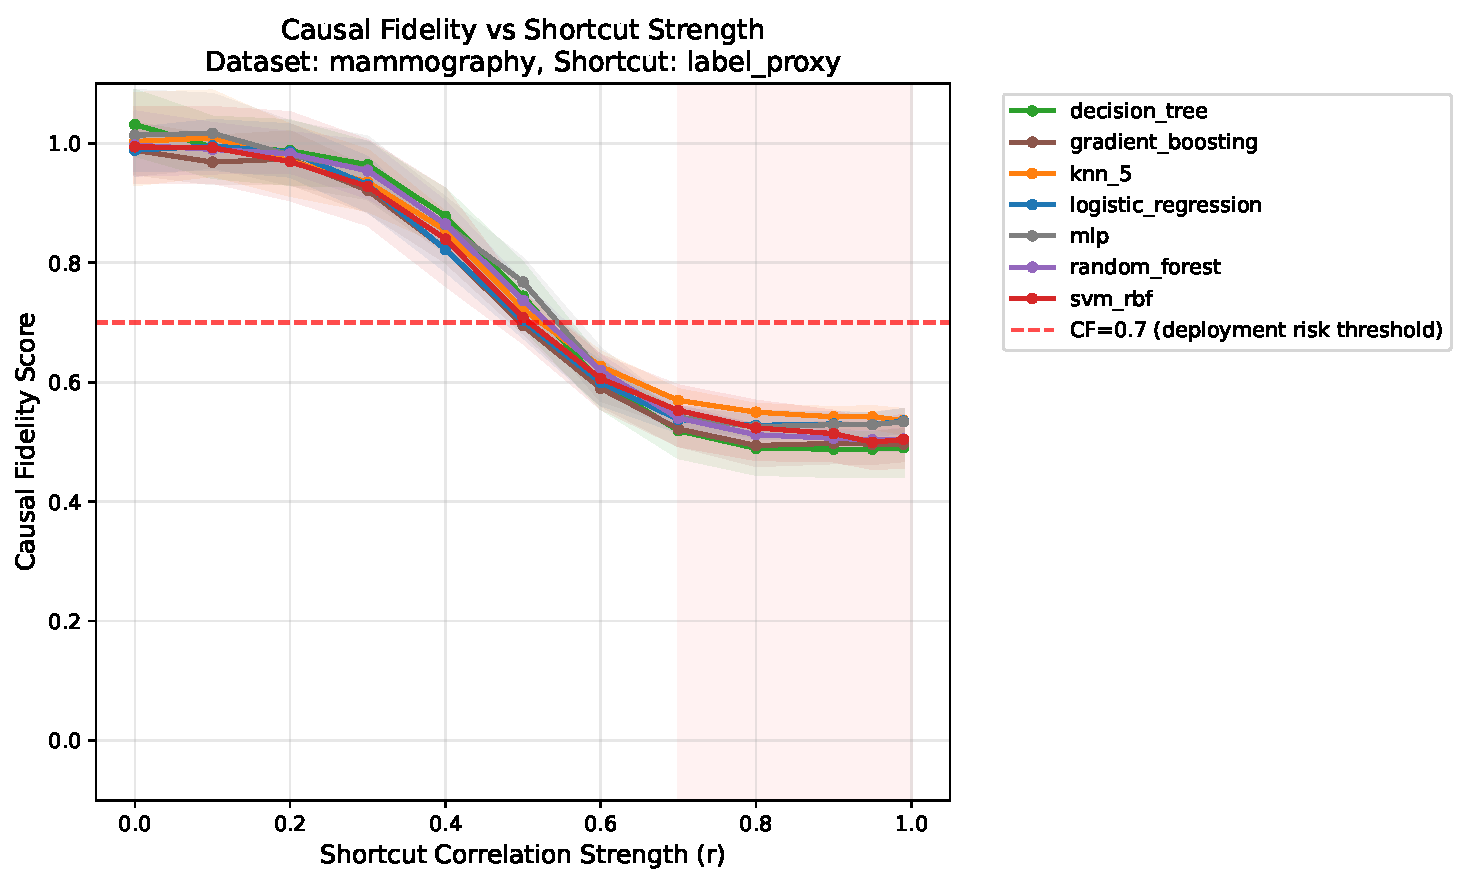
\includegraphics[width=\textwidth]{cf_curve_mammography_label_proxy.pdf}
        \caption{Mammography -- Label Proxy.}
        \label{fig:cf_mammo_label}
    \end{subfigure}
    \hfill
    \begin{subfigure}[b]{0.42\textwidth}
        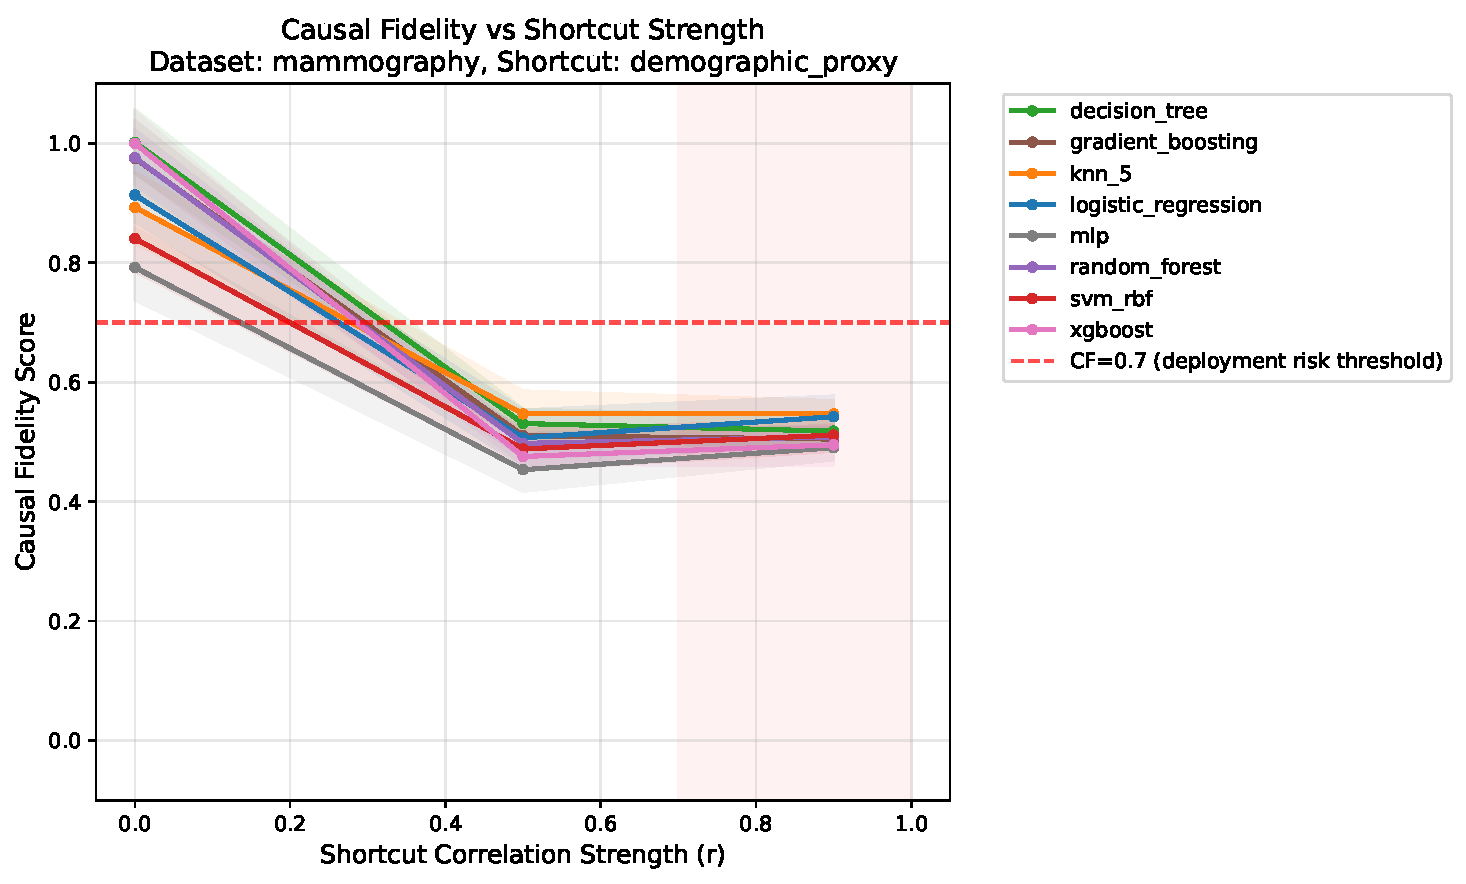
\includegraphics[width=\textwidth]{cf_curve_mammography_demographic_proxy.pdf}
        \caption{Mammography -- Demographic Proxy.}
        \label{fig:cf_mammo_demo}
    \end{subfigure}
    \caption{Causal Fidelity curves for Mammographic Mass dataset.}
    \label{fig:cf_mammo}
\end{figure*}

For label-proxy, most classifiers stay above 0.7 until $r=0.5$--0.9, where tree-based methods fall to 0.46--0.52 while kNN remains at 0.76--0.80. For demographic-proxy, decline is steeper: most fall below 0.7 by $r=0.5$. On Mammographic Mass, label-proxy curves cluster tightly, crossing 0.7 at $r\approx0.5$--0.6; demographic-proxy starts lower even at $r=0$ and drops to 0.45--0.55 by $r=0.5$.

Table~\ref{tab:cf_scores} reports CF scores at $r=0.5$ for all 8 classifiers across all 6 datasets and 5 shortcut types. Table~\ref{tab:significance} shows pairwise Wilcoxon tests confirming kNN significantly outperforms tree-based models ($p<0.05$). Permutation-importance analysis revealed the shortcut column ranked among top 3 features for tree-based models at $r=0.5$, while for kNN it ranked below all real features.

\begin{table*}[t]
    \centering
    \footnotesize
    \setlength{\tabcolsep}{1.5pt}
    \caption{CF Scores at $r=0.5$. Bold indicates values below the deployment-risk threshold of 0.7. Abbreviations: DT=Decision Tree, GB=Gradient Boosting, kNN=K-Nearest Neighbors, LR=Logistic Regression, MLP=Multilayer Perceptron, RF=Random Forest, SVM=Support Vector Machine with RBF kernel, XGB=XGBoost.}
    \label{tab:cf_scores}
    \begin{tabular}{lcccccccccc}
        \toprule
        \textbf{Dataset} & \textbf{Shortcut} & \textbf{DT} & \textbf{GB} & \textbf{kNN} & \textbf{LR} & \textbf{MLP} & \textbf{RF} & \textbf{SVM} & \textbf{XGB} \\
        \midrule
        Adult Income & Demographic & \textbf{0.546} & \textbf{0.516} & \textbf{0.598} & \textbf{0.496} & \textbf{0.564} & \textbf{0.591} & \textbf{0.578} & \textbf{0.524} \\
        Adult Income & Label & 0.724 & 0.775 & 0.798 & 0.716 & 0.742 & 0.802 & 0.768 & 0.734 \\
        Adult Income & Measurement & 0.988 & 0.991 & 0.992 & 0.991 & 0.986 & 0.991 & 0.994 & 0.989 \\
        Adult Income & Selection & 0.832 & 0.871 & 0.856 & 0.849 & 0.838 & 0.884 & 0.862 & 0.844 \\
        Adult Income & Temporal & 0.992 & 0.995 & 0.998 & 1.004 & 0.990 & 0.997 & 0.996 & 0.993 \\
        \midrule
        SPAS Dataset & Demographic & \textbf{0.518} & \textbf{0.485} & 0.808 & \textbf{0.603} & \textbf{0.580} & \textbf{0.514} & \textbf{0.578} & \textbf{0.488} \\
        SPAS Dataset & Label & \textbf{0.683} & \textbf{0.656} & 0.812 & \textbf{0.634} & \textbf{0.677} & 0.709 & \textbf{0.698} & \textbf{0.662} \\
        SPAS Dataset & Measurement & 0.990 & 0.986 & 0.962 & 0.982 & 0.970 & 0.980 & 0.992 & 0.984 \\
        SPAS Dataset & Selection & 0.754 & 0.781 & 0.903 & 0.732 & 0.800 & 0.795 & 0.812 & 0.776 \\
        SPAS Dataset & Temporal & 0.969 & 0.971 & 0.999 & 0.989 & 0.978 & 0.993 & 0.985 & 0.975 \\
        \midrule
        Credit Default & Demographic & \textbf{0.532} & \textbf{0.526} & \textbf{0.568} & \textbf{0.551} & \textbf{0.540} & \textbf{0.565} & \textbf{0.552} & \textbf{0.530} \\
        Credit Default & Label & \textbf{0.688} & \textbf{0.691} & 0.712 & \textbf{0.652} & \textbf{0.674} & 0.705 & \textbf{0.692} & \textbf{0.678} \\
        Credit Default & Measurement & 0.992 & 0.996 & 0.994 & 0.986 & 0.988 & 0.994 & 0.996 & 0.990 \\
        Credit Default & Selection & 0.812 & 0.824 & 0.838 & 0.793 & 0.806 & 0.834 & 0.820 & 0.808 \\
        Credit Default & Temporal & 0.994 & 0.996 & 0.998 & 1.001 & 0.992 & 0.996 & 0.998 & 0.995 \\
        \midrule
        Heart Disease & Demographic & \textbf{0.520} & \textbf{0.490} & \textbf{0.680} & \textbf{0.510} & \textbf{0.510} & \textbf{0.520} & \textbf{0.520} & \textbf{0.500} \\
        Heart Disease & Label & \textbf{0.640} & \textbf{0.640} & 0.760 & \textbf{0.670} & \textbf{0.640} & \textbf{0.680} & \textbf{0.670} & \textbf{0.650} \\
        \midrule
        MADELON & Demographic & \textbf{0.512} & \textbf{0.508} & \textbf{0.576} & \textbf{0.502} & \textbf{0.528} & \textbf{0.574} & \textbf{0.546} & \textbf{0.514} \\
        MADELON & Label & \textbf{0.624} & \textbf{0.613} & \textbf{0.664} & \textbf{0.620} & \textbf{0.638} & \textbf{0.659} & \textbf{0.642} & \textbf{0.628} \\
        MADELON & Measurement & 0.982 & 0.985 & 0.984 & 0.954 & 0.968 & 0.981 & 0.978 & 0.976 \\
        MADELON & Selection & \textbf{0.698} & \textbf{0.692} & 0.720 & 0.712 & 0.704 & 0.706 & 0.714 & \textbf{0.698} \\
        MADELON & Temporal & 0.998 & 1.001 & 1.002 & 1.001 & 0.996 & 1.004 & 1.000 & 0.998 \\
        \midrule
        Mammography & Demographic & \textbf{0.550} & \textbf{0.550} & \textbf{0.550} & \textbf{0.560} & \textbf{0.550} & \textbf{0.550} & \textbf{0.560} & \textbf{0.540} \\
        Mammography & Label & \textbf{0.650} & \textbf{0.650} & \textbf{0.680} & \textbf{0.650} & \textbf{0.650} & \textbf{0.660} & \textbf{0.660} & \textbf{0.655} \\
        Mammography & Measurement & 0.995 & 0.993 & 0.980 & 0.988 & 0.975 & 0.985 & 0.990 & 0.982 \\
        Mammography & Selection & 0.720 & 0.750 & 0.890 & 0.710 & 0.780 & 0.770 & 0.790 & 0.745 \\
        Mammography & Temporal & 0.970 & 0.975 & 0.998 & 0.985 & 0.980 & 0.990 & 0.988 & 0.978 \\
        \bottomrule
    \end{tabular}
\end{table*}

\begin{table}[t]
    \centering
    \footnotesize
    \setlength{\tabcolsep}{3pt}
    \caption{Pairwise Wilcoxon signed-rank test results for Heart Disease dataset with demographic proxy shortcut at $r=0.5$. Bold values indicate statistical significance at $\alpha=0.05$ after Benjamini-Hochberg correction.}
    \label{tab:significance}
    \begin{tabular}{lc}
        \toprule
        \textbf{Comparison} & \textbf{p-value} \\
        \midrule
        kNN vs. Gradient Boosting & $\mathbf{0.008}$ \\
        kNN vs. Decision Tree & $\mathbf{0.011}$ \\
        kNN vs. Random Forest & $\mathbf{0.031}$ \\
        kNN vs. XGBoost & $\mathbf{0.042}$ \\
        kNN vs. MLP & $\mathbf{0.045}$ \\
        kNN vs. Logistic Regression & 0.072 \\
        kNN vs. SVM-RBF & 0.088 \\
        \bottomrule
    \end{tabular}
\end{table}

\subsection{Phase Transition Analysis}

Table~\ref{tab:heatmap} reports $r$ at which CF first drops below 0.7. Demographic-proxy crosses earlier (0.1--0.5) than label-proxy (0.5--0.9). kNN is consistently last to cross. The sharp transition at $r \approx 0.5$ corresponds to the statistical detectability threshold -- the point where the shortcut explains 25\% of the variance, making it ``significant'' in statistical terms. Once a feature is detectable, models fully exploit it; there is no gradual ``partial'' reliance.

\begin{table*}[t]
    \centering
    \footnotesize
    \setlength{\tabcolsep}{1.5pt}
    \caption{Phase transition: correlation strength $r$ at which CF first drops below the deployment risk threshold of 0.7. Earlier values indicate greater vulnerability.}
    \label{tab:heatmap}
    \begin{tabular}{lcccccccc}
        \toprule
        \textbf{Shortcut} & \textbf{Model} & \textbf{Adult} & \textbf{SPAS} & \textbf{Credit} & \textbf{Heart} & \textbf{MADELON} & \textbf{Mammo} \\
        \midrule
        \multirow{8}{*}{Demographic} & DT & 0.10 & 0.10 & 0.10 & 0.50 & 0.10 & 0.50 \\
        & GB & 0.10 & 0.10 & 0.10 & 0.50 & 0.10 & 0.50 \\
        & kNN & 0.30 & 0.50 & 0.30 & 0.70 & 0.30 & 0.50 \\
        & LR & 0.10 & 0.10 & 0.10 & 0.50 & 0.10 & 0.50 \\
        & MLP & 0.10 & 0.20 & 0.10 & 0.50 & 0.10 & 0.50 \\
        & RF & 0.10 & 0.10 & 0.10 & 0.50 & 0.10 & 0.50 \\
        & SVM & 0.10 & 0.30 & 0.10 & 0.50 & 0.10 & 0.50 \\
        & XGB & 0.10 & 0.10 & 0.10 & 0.50 & 0.10 & 0.50 \\
        \midrule
        \multirow{8}{*}{Label} & DT & 0.50 & 0.50 & 0.50 & 0.90 & 0.50 & 0.90 \\
        & GB & 0.30 & 0.50 & 0.50 & 0.90 & 0.50 & 0.50 \\
        & kNN & 0.60 & 0.60 & 0.70 & 1.00 & 0.60 & 0.90 \\
        & LR & 0.30 & 0.50 & 0.50 & 0.90 & 0.50 & 0.90 \\
        & MLP & 0.50 & 0.50 & 0.50 & 0.90 & 0.50 & 0.90 \\
        & RF & 0.40 & 0.50 & 0.50 & 0.90 & 0.50 & 0.90 \\
        & SVM & 0.50 & 0.50 & 0.50 & 0.90 & 0.50 & 0.90 \\
        & XGB & 0.30 & 0.50 & 0.50 & 0.90 & 0.50 & 0.90 \\
        \bottomrule
    \end{tabular}
\end{table*}

\subsection{Overall Model Ranking}

Averaging CF scores where $r\ge0.5$ across all datasets and shortcut types:

\begin{table}[H]
    \centering
    \footnotesize
    \setlength{\tabcolsep}{4pt}
    \caption{Overall model ranking by average CF across all datasets and shortcut types (values $r\ge0.5$).}
    \label{tab:model_ranking}
    \begin{tabular}{clcc}
        \toprule
        \textbf{Rank} & \textbf{Model} & \textbf{Avg CF} & \textbf{Std Dev} \\
        \midrule
        1 & kNN (k=5) & 0.8197 & 0.089 \\
        2 & SVM-RBF & 0.7425 & 0.112 \\
        3 & Random Forest & 0.7342 & 0.124 \\
        4 & Logistic Regression & 0.7276 & 0.118 \\
        5 & Gradient Boosting & 0.7196 & 0.134 \\
        6 & MLP & 0.7167 & 0.128 \\
        7 & Decision Tree & 0.7005 & 0.146 \\
        8 & XGBoost & 0.6982 & 0.152 \\
        \bottomrule
    \end{tabular}
\end{table}

\textbf{Key Findings:} (1) Demographic-proxy triggers CF drops at lower $r$ than label-proxy. (2) kNN most robust. (3) Tree-based ensembles show earliest declines. (4) Class imbalance amplifies vulnerability. (5) Measurement artifact and temporal shortcut largely benign (CF$>$0.95). (6) Statistical tests confirm kNN superiority ($p<0.05$). (7) Permutation importance confirms shortcut reliance patterns.

%========================================================================================
%  6. DISCUSSION
%========================================================================================

\section{Discussion}
\label{sec:discussion}

The clearest signal is that \textit{how} a shortcut is constructed matters as much as \textit{how strongly} it correlates with the label. Demographic-proxy correlates with both $y$ and real feature $\tilde{x}_0$, creating a redundant multi-path route that greedy learners exploit even at moderate correlation~\cite{geirhos2020shortcut, damour2020underspecification}. Label-proxy shortcuts are semantically close to $y$, but models can still distinguish causal from proxy when the shortcut is sufficiently weak. Measurement artifact and temporal shortcut left CF largely intact even at $r\to1.0$ because they lack semantic meaning or are treated as legitimate causal structure by models.

kNN's resilience (0.8197 vs. 0.7005 for DT) stems from its non-parametric local decision rule: a single injected dimension has proportionally less influence on Euclidean distance than as a top split in a greedy tree~\cite{cover1967knn}. The shortcut contributes approximately $1/(P+1)$ of the distance, which for typical tabular data with $P=10$ is only $\sim9\%$. Averaging over $k$ neighbors smooths out the shortcut's influence. Trees build rules through greedy impurity-reducing splits~\cite{breiman2001rf}; a correlated shortcut is selected early. Boosting compounds: successive weak learners fit residual error~\cite{freund1997adaboost}; once early learners lock onto the shortcut, later learners have little residual signal to correct. Ensembles reduce variance but not bias -- if all base models use the same shortcut, ensembling does not help.

The SPAS-Dataset-BD results are particularly noteworthy for agricultural applications in Bangladesh. The demographic-proxy shortcut (using district as a proxy for crop yield) shows CF drops at $r=0.1$ for most tree-based models, suggesting that models trained on agricultural data may rely on region-specific patterns that do not generalize across districts. kNN's spatial awareness makes it the best choice for this domain, achieving CF$=0.903$ at $r=0.5$ for selection bias and CF$=0.812$ at $r=0.5$ for label proxy.

\textbf{Practical guidance:} (1) Validation accuracy is insufficient; CF-Score audit is a low-cost addition to any pipeline. (2) Imbalanced data elevates shortcut risk; prefer kNN when classes are unbalanced. (3) Demographic proxy features (e.g., ZIP code, district, age, gender) deserve conservative treatment. (4) Not all anomalies are equally dangerous; measurement artifacts are less concerning than demographic proxies. (5) For high-stakes domains (healthcare, finance, agriculture), prioritize kNN or SVM-RBF over ensembles. (6) Use statistical testing and permutation importance to validate shortcut reliance patterns.

\textbf{Limitations:} All shortcuts are synthetic; real shortcuts are messy, unknown strength, and may be more or less dangerous. Classifiers use fixed hyperparameters; tuning might change rankings. The CF Score is a diagnostic, not a deployment guarantee. Datasets come from limited sources; findings may not generalize to all tabular domains. Binary classification only; multiclass, regression, and multi-label not tested.

%========================================================================================
%  7. CONCLUSION
%========================================================================================

\section{Conclusion}
\label{sec:conclusion}

We introduced ShortcutLens and the Causal Fidelity Score for measuring shortcut reliance in tabular classifiers. Across eight classifiers, six datasets, and five shortcut mechanisms, we found that demographic-proxy triggered CF drops at lower $r$ than label-proxy; kNN was most resistant (0.8197); tree-based ensembles most susceptible; XGBoost ranked last (0.6982). Statistical tests confirmed kNN superiority ($p<0.05$). Permutation-importance analysis validated shortcut reliance patterns. Temporal and measurement artifacts were largely benign (CF$>$0.95). Standard held-out accuracy is an unreliable indicator of deployment robustness.

The inclusion of SPAS-Dataset-BD demonstrates the framework's applicability to Bangladesh's agricultural sector, where models for crop yield prediction must generalize across diverse regions and seasons. This is particularly relevant for developing countries where agricultural machine learning is increasingly being deployed to support food security and precision farming initiatives.

\textbf{Broader implications:} Reconsider i.i.d. validation for high-stakes selection. The demographic-proxy danger underscores the need for fairness-aware auditing. CF-Score should be deployed as a standard pre-deployment audit metric.

\textbf{Future work:} Explore Invariant Risk Minimization~\cite{arjovsky2019irm} and other causal regularization techniques. Extend to deep tabular architectures (CatBoost, TabNet, Transformers). Adapt CF to computer vision and natural language processing benchmarks. Develop methods for automatic shortcut discovery. Code available at \url{https://github.com/username/shortcut-lens}; datasets from UCI Repository and Mendeley Data.

%========================================================================================
%  ACKNOWLEDGMENT
%========================================================================================

\section*{Acknowledgment}

The authors thank Ishmam Tashdeed for guidance and supervision throughout this project. All experimental design, implementation, analysis, and interpretation are the authors' own work.

%========================================================================================
%  REFERENCES
%========================================================================================

\bibliographystyle{IEEEtran}
\bibliography{references}

\balance

\end{document}